\documentclass[conference]{IEEEtran}
\IEEEoverridecommandlockouts
% The preceding line only needs to identify funding in the first footnote. If that is unnecessary, please comment.
\usepackage{cite}
\usepackage{amsmath,amssymb,amsfonts}
\usepackage{algorithmic}
\usepackage{graphicx}
\usepackage{textcomp}
\usepackage{xcolor}
\usepackage{balance}
\usepackage{makecell}
\usepackage{hyperref}
\usepackage{url} %for URLs
\usepackage{listings} %for code
\usepackage{float}

%% Code listing style set
\lstset{frame=none,
%   language=SQL,
  aboveskip=3mm,
  belowskip=3mm,
  showstringspaces=false,
  columns=flexible,
  basicstyle={\small\ttfamily},
  numbers=none,
  numberstyle=\tiny\color{gray},
  keywordstyle=\color{blue},
  commentstyle=\color[rgb]{0,0.4,0}, 
  stringstyle=\color{purple},
  breaklines=true,
  breakatwhitespace=true,
  tabsize=4
}


\usepackage[letterpaper,%
            left=0.75in,right=0.75in,top=0.75in,bottom=1in,%
            footskip=.25in,bindingoffset=0.2in]{geometry}

\def\BibTeX{{\rm B\kern-.05em{\sc i\kern-.025em b}\kern-.08em
    T\kern-.1667em\lower.7ex\hbox{E}\kern-.125emX}}

\setlength{\columnsep}{0.25in}


\begin{document}

\makeatletter
\newcommand{\linebreakand}{%
 \end{@IEEEauthorhalign}
 \hfill\mbox{}\par
 \mbox{}\hfill\begin{@IEEEauthorhalign}
}
% \makeatother

\title{DW for Machine Learning Modelling of Algorithmic Trading Stocks-Price Prediction on DRI Hosting
}
% \footnote {\color{red} Gaétan: 1. Why does {\em title}
% need to mention the ETL stages? Why does it need to mention DRI in the title? How many readers will know what DRI is? 3. Why be specific about XGBoost in the title? 4. Why just mention "training results" while there are (a) training / inference results (b) precision of inference (c) speed of training / inference (d) scalability of training / inference? All those details should be part of the paper and the title should look more like "Precision, speed and scalability of algorithmic trading stocks-price prediction". Such a title really brings out the value of this workpackage without excessive details that can be made precise in the paper. }

% ======= Review 1 =======

% *** Guidance: Please provide specific recommendations that you would like to suggest to the author for improving the paper.

% 1. Describe your contributions beyond explaining what was built.
% The study provides an in-depth explanation of Cloud/HPC resources and automated pipelines; however, the research contribution will be clearer if the authors explain how their research expands upon prior ETL/ELT automation studies used in Algorithmic Trading Systems.

% 2. Expand on how the system performs forecasting.
% XGBoost based forecasting was noted in the paper, yet no quantitative predictive results were presented (i.e., accuracy, error rates, backtest results). Presenting some form of preliminary forecasting results will greatly enhance the paper.

% 3. Reduce amount of detail regarding Resource Allocation.
% The many descriptions of allocated CPU/GPU/storage resources, although useful information, dominate the narrative. The material contained in this section could be reduced to give more space to describe the design decisions made for the system, lessons learned regarding scalability and architectural trade-off decisions.

% 4. Provide more Reproducibility Guidance.
% The inclusion of code snippets and reference to a GitHub repository are very helpful; however, the paper would be enhanced with a single subsection which describes how the system can be recreated/adapted by others (dependencies, configuration assumptions, etc.).

% 5. Expand on Data Quality Issues and Imputation Strategy.
% The discussion of missing data handling states that there is a need for additional research into imputation methodologies. A high-level description or rationale for the interim methodology selections would add to the completeness of the methodology.

% 6. Streamline Organization and Remove Redundancy.
% Many of the sections provide similar explanations for why large datasets and automation are needed. By removing redundant explanations the reader will find the study easier to read and follow.

% *** Appropriate: Is the content appropriate for the conference themes?
% Very relevant (4)

% *** Content: How would you rate the quality of the technical/management content of the paper?
% Good (3)

% *** Recommendation: Do you recommend acceptance or rejection?
% Weak Accept (4)

% ======= Review 2 =======

% *** Guidance: Please provide specific recommendations that you would like to suggest to the author for improving the paper.

% Make clear the ML forecasting process and results
% Though the paper describes the data collection process, automation of ELT, as well as infrastructure design, the ML result for the forecasting process is barely mentioned. A section for experimental results or more detailed performance measures for the ML part could be added for further enhancement.

% "Improve separation between system engineering and ML contributions."
% Manuscript content is skewed towards system architecture and automation. A clear definition of system/ML-oriented work would be helpful in distinguishing it from other streams of work being done by other papers.

% Describe scalability limitations and fault tolerance
% Although system design is good, a short discussion about bottlenecks (API rate limiting, DB contention, network errors) and how to address them would make the system design review more robust. Make a brief comparison to existing ETL or ELT frameworks. The literature review is excellent; a table summarizing comparisons between this proposed method and more conventional ETL solutions (like Airflow-based pipelines) would be an improvement. It is now evident that O-RAN compliant networks will be essential for NB Minor editorial changes Some parts of the document could be shortened. Some light polishing of the language and some formatting issues (listings and ref figures) could help.

% *** Appropriate: Is the content appropriate for the conference themes?
% Moderately relevant (3)

% *** Content: How would you rate the quality of the technical/management content of the paper?
% Good (3)

% *** Recommendation: Do you recommend acceptance or rejection?
% Weak Accept (4)

% ======= Review 3 =======

% *** Guidance: Please provide specific recommendations that you would like to suggest to the author for improving the paper.

% The paper focus on automating data collection for algorithmic trading. The development work to build a reliable data pipeline is explained in detail.

% To improve the paper I would like to suggest the following specific recommendations for the author:
% 1. The main weakness of the paper is the complete absence of ML results. The title and abstract expects this is a system for "Machine Learning Modelling and Forecasting," but the paper only describes the data collection and transformation part.
% 2. The paper's novelty is not clearly mentioned. The use of Python, systemd, and PostgreSQL for data collection is a standard and well-established practice. This paper should clarify what makes this work novel. Is it the architecture, the amount of the data used, a unique solution to a specific problem in financial data collection, or the combination of these elements? The main contributions listed in the introduction should be revisited to highlight what is genuinely new to the research community.
% 3. The literature review sections mentions only about the authors' previous publications. While it is important to build on prior work. I would recommend including a more critical review of recent, relevant papers from other research groups to better position the contribution of this work.
% 4. The conclusion mentions about findings related to the ML model that are not presented in the paper.
% 5. The Future work is also not mentioned in the paper

% *** Appropriate: Is the content appropriate for the conference themes?
% Highly relevant (5)

% *** Content: How would you rate the quality of the technical/management content of the paper?
% Fair (2)

% *** Recommendation: Do you recommend acceptance or rejection?
% Weak Reject (2) 
\author{

     
    % \IEEEauthorblockN{Justin Drenka}
    % \IEEEauthorblockA{\textit{Computer Science} \\
    % \textit{UBCO}\\
    % Kelowna, Canada \\
    % 0009-0008-6821-8379}

    % \and

    % \IEEEauthorblockN{Helana Jaraiseh}
    % \IEEEauthorblockA{\textit{Computing Science} \\
    % \textit{UFV}\\
    % Abbotsford, Canada \\
    % 0009-0000-1239-2820}

    % \and


\IEEEauthorblockN{Emilio}
    \IEEEauthorblockA{\textit{Computer Science} \\
    \textit{Okanagan College}\\
    Kelowna, Canada \\ }
    
    \and
    
   
    \IEEEauthorblockN{Kristina CORMIER}
    \IEEEauthorblockA{\textit{Computer Science} \\
    \textit{Okanagan College}\\
    Kelowna, Canada \\
    0009-0004-3783-9704} 

\and 

    \IEEEauthorblockN{Harsh}
    \IEEEauthorblockA{\textit{Computer Science} \\
    \textit{Okanagan College}\\
    Kelowna, Canada \\
    }

    
    % \and
    
    % \IEEEauthorblockN{Youry Khmelevsky}
    % \IEEEauthorblockA{\textit{Computer Science} \\
    % \textit{Okanagan College}\\
    % Kelowna, Canada \\
    % 0000-0002-6837-3490}
    
    % \and
    % \IEEEauthorblockN{Ga\'etan Hains}
    % \IEEEauthorblockA{ \textit{LACL} \\
    % \textit{Université Paris-Est}\\
    % Créteil, France \\
    % 0000-0002-1687-8091} 

    % \and
    
    % \IEEEauthorblockN{Albert Wong}   \IEEEauthorblockA{\textit{Mathematics and Statistics} 
    % \\\textit{Langara College}\\
    % Vancouver, Canada \\
    % 0000-0002-0669-4352}



% \and 
%     \IEEEauthorblockN{Frank Zhang}
%     \IEEEauthorblockA{\textit{School of Computing} \\
%    \textit{University of the Fraser Valley}\\
%    Abbotsford, Canada \\
%     0000-0001-7570-9805}   
}

\maketitle

%%%%%%%%%%%%% AI Guidelines for AI-Generated Content %%%

% see more here: https://conferences.ieeeauthorcenter.ieee.org/author-ethics/guidelines-and-policies/submission-policies/#:~:text=1.,review%20for%20another%20refereed%20publication.

% IEEE Guidelines for AI-Generated Content

% The use of Artificial Intelligence (AI) and large-scale language models (LLMs) in paper submissions is governed by specific rules. 

% Disclosure is Mandatory: The use of AI-generated text or Content (including text, figures, images, and code) must be disclosed in the acknowledgments section of the paper. The specific AI system used and the sections where it was used should be identified.

% Editing vs. Content Generation:

% Allowed (with recommended disclosure): Using AI for basic editing, grammar enhancement, or translation is standard practice and generally allowed, though disclosure is recommended.

% Prohibited (unless part of analysis): Submissions that include significant, unattributed AI-generated text as the core content of the work are prohibited unless the AI's output itself is the subject of the paper's experimental analysis.

% Author Responsibility: Authors remain fully responsible for the correctness, originality, and veracity of all submitted Content, including checking for plagiarism and "hallucinations" from AI tools. 
%%%%%%%%%%%%%%%%%%%%%%%%%%%%


\begin{abstract}
% This research paper focuses on developing an automated data collection and transformation framework for Algorithmic Trading (AT) forecasting using machine learning (ML). The implementation of the computational resources is supported by a grant from the Digital Research Alliance of Canada (DRAC), Alliance Cloud Connect Pilot \cite{DRI}. This enables large-scale data processing, storage, and model training. Historical market data and real-time data streams are collected at 5-minute intervals, stored in staging tables of a PostgreSQL DBMS, and aggregated into 15-minute intervals in a custom-built Data Warehouse. It is essential to ensure that data from multiple sources remains consistent, accurate, and reliably reproducible throughout the data pipeline.  

\end{abstract}

\begin{IEEEkeywords}
Algorithmic Trading, Machine Learning Modelling, System Integration, Performance Optimization, High Performance Computing, Advanced Research Computing, Research Data Management
\end{IEEEkeywords}

\section{Introduction}

% \setlength{\fboxrule}{2pt}
%     	\fcolorbox{red}{white}{
%         	\parbox{0.8\linewidth}{
%          -- This is your  ``business case" of your project. \\
%          -- You can read all introductions in all AlgTr papers and summarize here.\\
%          -- Please add non-functional and functional requirements. \\
%          -- Please add ultimate goals for the project here (3 sunbeams — at least 3 goals).\\
%          -- Ultimately, we should have 2-3 new planned novelties/achievements from the project (!!!).\\
%          -- Ultimately, you need 1-3 pages for this. \\
%         	}
%         }\\


While short-term predictive modeling is foundational to data-intensive infrastructures such as smart grids and supply chain logistics, its deployment in financial time-series forecasting represents a sophisticated frontier for high-frequency risk mitigation and autonomous decision-making \cite{fischer2018deep, ghoddusi2019machine}. When systems process structured data at high frequency, delayed decisions can directly erode economic performance, weaken system stability, and amplify operational risks \cite{lim2021time}. Minor improvements in the predictive performance of short-term models may translate into measurable competitive advantages, ranging from increased trading yields to optimized resource utilization \cite{gu2020empirical,mullainathan2017machine}. Building machine learning frameworks that achieve both computational scalability and predictive robustness for short-horizon forecasting is therefore a critical technical and economic objective \cite{chen2016xgboost, drac2024infrastructure, gu2020empirical}. 

Advances in ensemble learning architectures have markedly enhanced the predictive capacity and generalization performance for tasks involving high-dimensional structured data \cite{chen2016xgboost}. With modern ML approaches, Gradient-Boosted Decision Trees (GBDT) frameworks consistently deliver robust predictive performance, especially in the face of the nonlinear dynamics and heterogeneous feature spaces that characterize financial time‑series data \cite{chen2016xgboost, friedman2001greedy}. Among these approaches, XGBoost has emerged as a widely adopted framework due to its regularization mechanisms, efficient parallel tree construction, and resilience to noisy structured datasets. Its scalability and computational optimizations make it particularly suitable for large-scale forecasting problems \cite{chen2016xgboost}. 

As data streams scale in both volume and frequency, they impose substantial challenges on system architecture, computation, and real‑time processing \cite{Stonebraker2005OneSize}. Deploying robust short-term forecasting models requires sophisticated pipelines that manage the end-to-end lifecycle—from ingestion to aggregation—leveraging the parallel processing capabilities of the Fir distributed cluster \cite{drac2024infrastructure, Colonnelli2021StreamFlow}. High-performance computing (HPC) infrastructures such as the Digital Research Alliance of Canada (DRAC) provide access to parallel processing, distributed storage, and scalable compute nodes, enabling large-scale machine learning experimentation. The system architecture adopts a distributed computing paradigm facilitated by the Fir cluster \cite{drac2026hpc}, ensuring that the ingestion and retraining pipelines remain efficient and parallelizable through parallelized execution across high-performance compute nodes \cite{chen2016xgboost}.

Prior studies in algorithmic trading and short-term forecasting (AlgTr) have demonstrated strong performance advantages of tree-based ensemble models over linear regression and baseline statistical approaches for structured financial time-series data \cite{fama1970efficient, hull2017options}. Collectively, these studies emphasize how feature construction, window‑based aggregation, and volatility‑aware metrics are essential for modeling complex financial time‑series \cite{lopezdeprado2018afml}. Nevertheless, many existing implementations assume relatively clean datasets, limited data volumes, or single-node training configurations \cite{widmer1996learning}. While machine learning applications on HPC have been explored in terms of individual performance and scalability aspects, comprehensive integration of HPC infrastructure with end-to-end data preprocessing, deduplication, and distributed training workflows remains underinvestigated \cite{lewis2025io, badia2024dagstuhl}.

Following the data preparation methodologies outlined by Aggarwal \cite{aggarwal2015datamining}, this project uses a custom preprocessing pipeline to filter transient anomalies and resolve timestamp inconsistencies before training our model on the Fir cluster. Failure to mitigate these data quality issues can introduce systemic bias into feature aggregation, lead to computational inefficiencies through redundant data, and ultimately degrade the generalization performance of the predictive model \cite{han2011datamining}. As dataset volumes reach the scale of millions, inadequate preprocessing and inadequate resource distribution can lead to prohibitive training times and excessive storage demands, necessitating a more robust distributed architecture \cite{chen2016xgboost, hwang2012distributed}. This motivates the development of a scalable, resource‑efficient short‑term prediction system that combines strong data preprocessing, optimized feature engineering, and distributed XGBoost training on HPC infrastructure \cite{raschka2019pythonml}. Beyond predictive performance, the framework must ensure efficient computation, rigorous reproducibility, and stability when operating under noisy or dynamically shifting data conditions \cite{peng2011reproducible}. 

To address these challenges, this project proposes the design and implementation of an end-to-end short-term prediction pipeline leveraging DRAC computational infrastructure and XGBoost modeling. The framework emphasizes efficient data ingestion, systematic deduplication, structured feature aggregation, and optimized distributed model training. The objective is to construct a reproducible and scalable system capable of handling high-frequency structured datasets while maintaining strong predictive performance and controlled computational costs.

From a system perspective, the proposed framework must satisfy several functional requirements. First, it must support large-scale data ingestion and incremental updates within a dimensional data warehouse architecture \cite{kimball2013dwtoolkit}. Second, it must incorporate automated duplicate detection and resolution mechanisms prior to model training \cite{aggarwal2015datamining}. Third, it must generate temporally aggregated features appropriate for short-horizon forecasting \cite{lopezdeprado2018afml}. Fourth, it must enable scalable model training and evaluation over warehouse-scale datasets using distributed computational resources \cite{chen2016xgboost}. Finally, it must produce short-term predictions within a defined prediction horizon and report standardized performance metrics \cite{fawcett2006roc}.

Beyond functional capabilities, the system must adhere to several non-functional requirements essential for operational viability in financial environments. Scalability is paramount; the ELT pipeline must ingest and transform millions of records into the data warehouse without linear performance degradation \cite{tsay2010financial}. Computational efficiency is strictly required to optimize the ML training phase and minimize resource footprint within the shared HPC environment \cite{chen2016xgboost}. Furthermore, the system must demonstrate robustness, maintaining predictive stability even when the data warehouse is subjected to the non-stationary distributions and 'concept drift' typical of high-frequency streams \cite{widmer1996learning}. To ensure scientific validity, reproducibility is integrated into the workflow, allowing for consistent model analysis across iterative experiments \cite{peng2011reproducible}. Finally, resource optimization is mandated to prevent storage bloat during the transformation phase and mitigate redundant computational overhead during distributed analysis \cite{hwang2012distributed}.

The goals of this project center on three core objectives. First, to design a scalable end‑to‑end short‑term prediction pipeline that integrates ELT processes, data‑warehouse operations, and distributed XGBoost training within HPC infrastructure. Second, to strengthen predictive stability and generalization when modeling high‑frequency, noisy structured data through systematic preprocessing and feature aggregation. Third, to improve computational efficiency and resource utilization across the ingestion, transformation, and distributed training stages, acknowledging the resource constraints inherent to shared HPC environments.

The planned contributions of this work can be articulated across three dimensions. First, it introduces a scalable preprocessing and deduplication architecture tailored to the demands of high‑frequency short‑term forecasting datasets. Second, it develops an optimized XGBoost training configuration designed for distributed execution on DRAC infrastructure, with an emphasis on effective resource allocation and parallel computation. Third, it integrates a unified evaluation framework that jointly assesses predictive accuracy, computational efficiency, and infrastructure utilization, thereby linking model‑level performance with system‑level optimization.

By unifying scalable data engineering, distributed training optimization, and robust short-term predictive modeling within a coherent framework, this work aims to contribute both methodological and systems-level advancements to short-horizon machine learning prediction.

The remainder of this paper is organized as follows. Section II describes the system architecture and data preprocessing pipeline. Section III presents the feature engineering methodology and model configuration. Section IV details the experimental setup and evaluation metrics. Section V discusses results and performance analysis. Finally, Section VI concludes the paper and outlines future work.


% The applied research paper discusses solutions for automatically acquiring complete historical and real-time datasets, as well as the significant storage and computational resources required to train a machine learning model for short-term Algorithmic Trading predictions. The focus during this phase of the project is on automating data collection and transformation. 

% The Alliance Cloud Connect Pilot allocated 200 core-years on the NIBI-compute system, 20.0 RGU-years on the nibi-gpu system, and 59 TB of project storage on the NIBI storage system for High Performance Computing (HPC). It also allocates 16 VCPU-years, 4 cloud instances, 32 GB of RAM, 7 volumes, 7 snapshots, 2 Floating IP addresses, and 60,000 GB of cloud volume and snapshot storage for the cloud allocations on the Arbutus-persistent-cloud system.

% After a project is approved and resources are allocated, a few more steps are required to access them. One of the first steps is to set up Secure Shell (SSH) keys to access the resources. Another critical step was to set up Multi-factor Authentication (MFA), which is used when signing in to DRAC and when using the SSH tunnel to access the server. Furthermore, users must email DRAC to request access to specific resources, specify the required quantity, and wait for a reply before connecting to the dedicated PostgreSQL database. 

%  With the provided resources, the data could be collected for the past thirty years. The previous work only included the three previous years. The new dataset is ten times larger than the previous datasets described in \cite{financialModelingPrep, Wong2022, Wong2023, wong2023short, Wong2023ShortTerm, Wong2023ForecastingModels, Khmelevsky2023DataExtraction}.

% One of our biggest challenges is that many previous datasets are incomplete, leading to unexpected results with machine learning models. The current work focuses on updating missing values and expanding the dataset obtained from the data sources automatically.

% The main contributions of this paper are (1) a new approach to data collection from external data sources for XGBoost training, testing, and stock forecasting; (2) the new and historical datasets uploaded to a PostgreSQL general purpose DBMS within DRI research project; and (3) the design and testing of a new API for direct access to the DBMS from the core subsystem as part of machine learning (ML) training, testing, and forecasting on the vast datasets collected, transformed, and stored in the DBMS. 


\section{Existing Works}
   	\fcolorbox{red}{white}{
        	\parbox{0.8\linewidth}{
        	-- Somebody should read already published Alg Trad. research papers and explain here what was done in 2-4 paragraphs  \\}
        }\\
        

This work is a continuation of the previous research projects described in \cite{
% Khmelevsky2009SWdev, Khmelevsky2009gis, 
Khmelevsky2010Cloud, Khmelevsky2011IntCollab, Khmelvesky2011ResTeaching, Khmelevsky2013Mobile, Khmelevsky2015hybrid, 
2015HainsCodeGenUML,
Khmelevsky2016TenYears, Khmelevsky2016sport, 
% Khmelevsky2016Anew, 
Khmelevsky2016biometric,
%Khmelevsky2017gis, 
Khmelevsky2017Bot,
Khmelevsky2017gaming, 2020HainsGamersNetPerf, 
Khmelevsky2020ML,
Wong2021Gamers
% ,Khmelevsky2023DW
} 

% In our previous papers, we analyzed existing work on algorithmic trading systems and ML algorithms for predicting stock prices, such as Al-Akashi and Hassan \cite{Al-Akashi2022}, Kolte et al. \cite{kolte2022}, and Li \cite{li2023}, and related statistical methods for prediction accuracy. R. K. Dubey in  “Algorithmic Trading: The Intelligent Trading Systems and Its Impact on Trade Size” \cite{Dubey2022} reported about ``lack of progress in developing an algorithmic trading system that is operationally efficient.'' ``The main issues remain in acquiring, transforming, and storing the large datasets required for such a system" \cite{Martinez2022}. Many algorithmic trading and ML forecasting projects were limited by the size of the data set during model development and by the lack of system support for implementing the developed models \cite{theate2021application}.

% Yulianto in \cite{yulianto2019extract} stressed that the ``heterogeneity of data from various sources can be dealt with by designing an Extract, Clean, Conform, and Delivery/Load" process. Azeroual et al.\cite{azeroual2019etl} stated that implementing the ETL process could overcome many current challenges in data analysis. Oyewale et al. \cite{oyewale2024} informed that ``market complexity and volatility, along with the volume and speed at which financial data is generated, shape the challenges surrounding stock market analysis." On the other hand, Haryono et al. \cite{haryono2020comparison} stressed that ``ETL (Extract/Transform/Load) and ELT (Extract/Load/Transform) are the primary data processing methods for implementing a DW." Katari and Rodwal \cite{katarinext} identified issues in traditional ETL processes in financial markets. Our research over the last few years has confirmed that the ELT process is preferable to ETL. 

% Patel et al. in \cite{patel2020progressive} outlined ETL tools, some of which are ``code-based, GUI-based, cloud-based, Metadata support, Real-time support, and batch processing. Michael et al. discuss ETL systems for building a DW in their research. Biswas et al. in \cite{biswas2020efficient} described commercially available GUI-based products as ETL solutions. Ali \cite{ali2018next} created an ETL framework for Big Data. On the other hand, relatively few papers investigate the complete data life cycle \cite{zhang2023}. Wu et al. \cite{Wu2023} proposed using Apache Airflow with Python scripts to automate ETL tasks. The previous analyses on several implementation techniques were documented in \cite{Khmelevsky2023DataExtraction}.

% Based on the described works above and our research team's testing and observations, we use a well-established, proven object-oriented approach to design an efficient ELT process for this research project. The Python scripts,  PostgreSQL DW, and a user interface (UI) are used to improve the performance of the ELT process.


%%%%%%%%%%%%%%%%%%%%%%
%Section III
%%%%%%%%%%%%%%%%%%%%%%
\section{Methodology and Project Design} \label{sec:DataCollection}

   	\fcolorbox{red}{white}{
        	\parbox{0.8\linewidth}{
        	-- Please try to put here everything that you have in your RFP and in the Elaboration.
        }\\
}
\section{Data Collection Automation using DRI Resources} \label{sec:DataCollection}

   	\fcolorbox{red}{white}{
        	\parbox{0.8\linewidth}{
        	- This is your SubTeam I Construction I and II reports.
        }\\
 }
 
\subsection{ Overview of the Auto Data Collector System}
% To achieve accurate short-term forecasting, the model must always be aware of recent market activity. The automated data collection system on Fig.~\ref{Automated Data Collector Architecture} is designed to provide this by continuously updating the model dataset with current market information. 

% auto collector diagram img
\begin{figure*}[ht]
    \centering
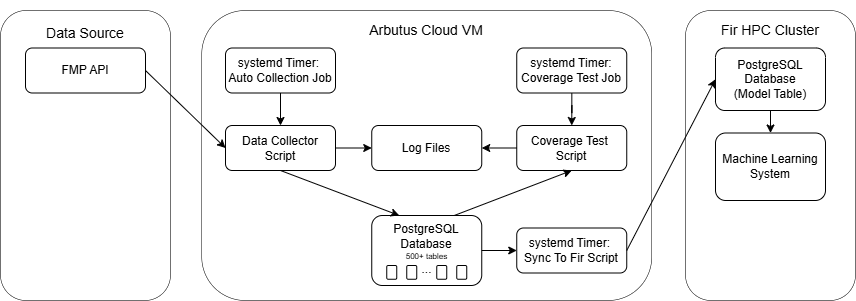
\includegraphics[width=0.75\textwidth]{images/newestcollectordiagram.png}
    \caption{Automated Data Collector Architecture and Workflow Design}
    \label{Automated Data Collector Architecture}
\end{figure*}


\subsection{ Cloud Deployment and Scheduling}

% The automated collector lives on a virtual machine instance within the Arbutus Cloud, part of Canada's Digital Research Infrastructure (DRI)\cite{DRI}. The system runs on a p4-6gb instance, which provides 4 virtual CPUs, 6 GB of RAM, and a 20 GB persistent disk. Hosting the process in the cloud enables consistent up-time, remote access, and protection against local hardware or power failures. Arbutus Cloud instances offer persistent storage, allowing the collector to run continuously without manual intervention. After about fifteen days of collection for 500 tickers, the PostgreSQL database uses roughly 100 MB of space, most of which is initial PostgreSQL table and index metadata rather than data records. This shows that the available storage is more than enough to support years of collected market data. 

% Job scheduling is managed using systemd timers, which run data collection at fixed intervals during standard market hours. This scheduling method ensures that no data is missed and that execution remains reliable in the event of a network or system interruption. Each run creates a status log, forming a history of performance for easy review and debugging. This combination of stable cloud infrastructure with automated scheduling supports a reliable data pipeline that stays synchronized with current market data and requires minimal operator oversight. 

% As shown in Listing~\ref{lst:collector_timer}, a \textit{systemd} timer deployed on the VM triggers the collector throughout standard stock market hours.

% \begin{lstlisting}[language=bash, caption={Systemd timer for the Auto Data Collector}, label={lst:collector_timer}]

% [Unit]
% Description=Auto Data Collector Timer

% # Run data collector twice per market hour
% # Time in UTC on the VM
% [Timer]
% OnCalendar=Mon..Fri *-*-* 13:58
% # Market open 09:30 EST
% OnCalendar=Mon..Fri *-*-* 14:30 
% OnCalendar=Mon..Fri *-*-* 14:58
% ...
% OnCalendar=Mon..Fri *-*-* 20:58
% # Market closed 16:00 EST
% OnCalendar=Mon..Fri *-*-* 21:30

% Persistent=true
% AccuracySec=1s

% [Install]
% WantedBy=timers.target
% \end{lstlisting}

The timer triggers the service shown in Listing~\ref{lst:collector_service}, which executes the collector script.

% \begin{lstlisting}[language=bash, caption={Systemd service that runs the Auto Data Collector}, label={lst:collector_service}]

% [Unit]
% Description=AutoDataCollector Service
% # Ensure network is ready before running
% After=network.target 

% [Service]
% # Run the script once per timer trigger
% Type=oneshot 
% User=almalinux
% WorkingDirectory=.../AutoDataCollector/
% # Entry script executed by the service
% ExecStart=.../bin/run_collector.sh
% # Retry if the script exits with an error 
% Restart=on-failure

% [Install]
% WantedBy=multi-user.target
% \end{lstlisting}


\subsection{ Data Collection Process }

% The automated data collection process is handled by a Python script that runs on the virtual machine described in Section B. The collection script is designed to be run continuously throughout standard trading hours. During each execution, a time window is created which covers the most recent trading period, with a slight overlap from the previous run to ensure no data is missed. As shown in Listing~\ref{lst:collector_window}, the script computes a rolling one-hour EST window that ends twenty minutes before the current time, creating deliberate overlap between runs to ensure that no time interval is ever missed. 

% \begin{lstlisting}[language=Python, caption={Time window calculation used by the Auto Data Collector}, label={lst:collector_window}]

% # Determine rolling 1-hour time window
% def get_current_time_window():
%     now_ny = datetime.now(ZoneInfo("America/New_York"))

%     # End window 20 minutes before now to ensure no missed rows from API
%     end_time = now_ny.replace(second=0, microsecond=0) - timedelta(minutes=20)
%     start_time = end_time - timedelta(hours=1)

%     # Store timestamps in EST 
%     return start_time.replace(tzinfo=None), end_time.replace(tzinfo=None)
% \end{lstlisting}

% Data is extracted from the Financial Modelling Prep (FMP) \cite{financialModelingPrep} API using this time window, and the schedule is configured so that each collection occurs shortly after new data becomes available. This keeps the database aligned with recent market activity with a slight lag. 

% The script uses lists of tickers so that symbols we want to track can be added or removed at any time, and the collector will adjust. This makes the system flexible and easier to maintain as data requirements evolve. Because FMP provides timestamps in EST, the script preserves this format when inserting records into the PostgreSQL database. After retrieving recent data from FMP, the results are written to the database with an ``upsert" operation, where entries are updated when already present, and inserted when not present yet. Listing~\ref{lst:collector_upsert} shows the portion of the collector that filters each record into the active time window and writes it to the corresponding ticker table using an UPSERT operation.

% \begin{lstlisting}[language=Python, caption={Filtering and UPSERT insertion of 5-minute records}, label={lst:collector_upsert}]

% # Fetch, filter, and upsert 5-minute market data into the staging table
% rows = []
% for record in data:
%     ts = parse_fmp_timestamp(record["date"])
%     if window_start <= ts < window_end and record.get("close") is not None:
%         rows.append((
%             ts, 
%             record["open"], 
%             record["high"],
%             record["low"], 
%             record["close"],
%             record["volume"]
%         ))

% sql = f"""
%     INSERT INTO {table} (ts, open, high, low, close, volume)
%     VALUES %s
%     ON CONFLICT (ts) DO UPDATE SET
%         open=EXCLUDED.open, high=EXCLUDED.high,
%         low=EXCLUDED.low, close=EXCLUDED.close,
%         volume=EXCLUDED.volume;
% """
% # Bulk insert all row tuples into DB
% execute_values(cursor, sql, rows)
% \end{lstlisting}
% % Running this process with \textit{systemd} timers on the cloud-based VM ensures a stable environment for collection, keeping the historical dataset up to date, accurate, and ready for training the forecasting model.

\subsection{ Database Storage Architecture }

% The auto collector stores new market data in a set of staging tables in the database, with each ticker getting its own table. Each table uses OHLCV format (open, high, low, close, and volume), matching the structure provided by our data source (FMP API). These values describe how the market price moved during each time interval, and using the same format as the historical dataset keeps both sources consistent. 

% Every entry in the staging tables represents one 5-minute interval and is identified by its timestamp. Listing~\ref{lst:staging_table} shows the structure of a typical staging table, where the timestamp serves as the primary key, ensuring that overlapping collection windows do not introduce duplicates.
% \begin{lstlisting}[language=SQL, caption={Example staging table used for a single ticker}, label={lst:staging_table}]
% -- Staging table for a single ticker (AAPL)
% CREATE TABLE IF NOT EXISTS market.aapl (
%     ts     TIMESTAMP PRIMARY KEY,
%     open   DOUBLE PRECISION,
%     high   DOUBLE PRECISION,
%     low    DOUBLE PRECISION,
%     close  DOUBLE PRECISION,
%     volume BIGINT
% );
% \end{lstlisting}
% Choosing the timestamp as the primary key allows the collector to easily update rows when collection windows overlap, and separating each ticker into its own table avoids write conflicts when many symbols are updated at the same time. This simple layout makes the storage layer easy to maintain and reliable for continuous data collection. 

% The staging tables serve as the first stop for new data. Their role is to hold recent market information in the same structure as the historical dataset. In a later step of the pipeline, both the historical data and the auto-collected staging data are combined into a single model table used for training the forecasting model. 
% % That merging process is described in section: todo: add correct section here

% \subsection{Testing and Logging}
% Testing and logging are essential to ensure the auto collector captures 100\% of the expected market data for each market day. The system includes a daily coverage test that runs automatically about one hour after the market closes. Its job is to check that every 5-minute interval during standard trading hours is collected for every ticker. 
% Commented, Youry, 1 Feb 2026 to reduce paper length. 

% Listing~\ref{lst:coverage_test} shows the core logic of the daily coverage test, which verifies that the expected number of 5-minute intervals was collected for each ticker.
% \begin{lstlisting}[language=Python, caption={Core logic of the daily coverage test}, label={lst:coverage_test}]
% # Single ticker coverage between two dates
% def coverage_for_symbol(conn, symbol, start_date, end_date):
%     expected_per_day = expected_intervals_per_day()
%     total_expected = 0
%     total_actual = 0

%     table = format_table_name(symbol)
%     current = start_date

%     with conn.cursor() as cur:
%         while current <= end_date:
%             # Skip weekends
%             if current.weekday() >= 5:
%                 current += timedelta(days=1)
%                 continue

%             # Intervals for one trading day
%             total_expected += expected_per_day

%             # Count found rows for that day
%             open_dt  = datetime.combine(current, time(9,30)).replace(tzinfo=None)
%             close_dt = datetime.combine(current, time(16,0)).replace(tzinfo=None)

%             cur.execute(
%                 f"SELECT COUNT(*) FROM {table} WHERE ts >= %s AND ts < %s",
%                 (open_dt, close_dt),
%             )
%             total_actual += cur.fetchone()[0]

%             current += timedelta(days=1)

%     # Return coverage percentage
%     return (total_actual / total_expected) * 100 if total_expected else 0
% \end{lstlisting}

% The test knows the collection start date and adjusts its expectations as days pass, so it continuously logs the coverage percentage for each ticker. This helped us catch several issues early, such as missing intervals, FMP API changes, and unexpected execution times. Finding these problems quickly made it much easier for us to ensure the dataset is complete and clean.

% In addition to the coverage test, the collector writes a status log for every scheduled run, noting when the job started, when it finished, how long it took and whether any errors occurred. The coverage test also records its results in the logs. Together, these tests and logs provide essential visibility into the system's performance and ensure its data remains accurate over time.

\section{API Architecture, Design and Testing to DRI DW}

\setlength{\fboxrule}{2pt}
    	\fcolorbox{red}{white}{
        	\parbox{0.8\linewidth}{
        	
            -- This is your Subteam II Construction I and II reports. \\
           }
        }\\

\subsection{Data Transformation for DW}

% \setlength{\fboxrule}{2pt}
%     	\fcolorbox{red}{white}{
%         	\parbox{0.8\linewidth}{
        	
%             -- Brandon\\
%             -- Youry, please review 2025-11-25
%            }
%         }\\
        
The transformed data gets inserted back into the database.

\subsection{DW and Staging Database Synchronization}

% \setlength{\fboxrule}{2pt}
%     	\fcolorbox{red}{white}{
%         	\parbox{0.8\linewidth}{
        	
%             -- James\\
%             -- Youry, please review 2025-11-27
%            }
%         }\\

\begin{figure*}[ht]
\centering
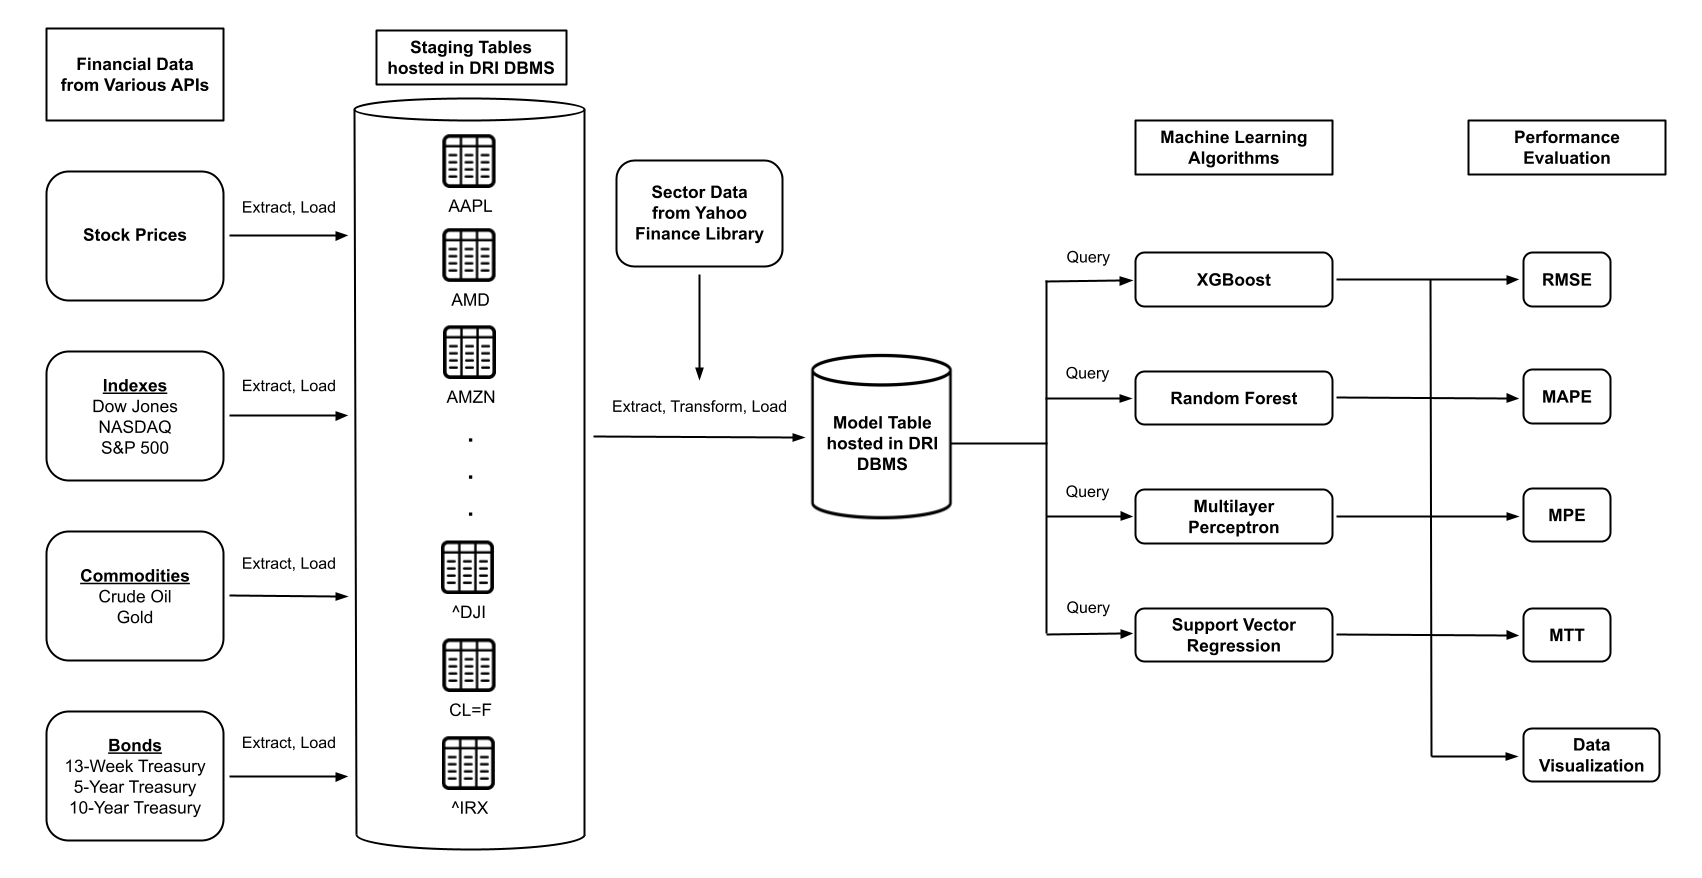
\includegraphics[width=0.75\textwidth]{images/Algorithmic Trading ELT-Automation-Architecture.png}
\caption{Automated ELT Architecture of the Algorithmic Trading System}
\label{fig: ETL}
\end{figure*}

\begin{figure*}[ht]
\centering
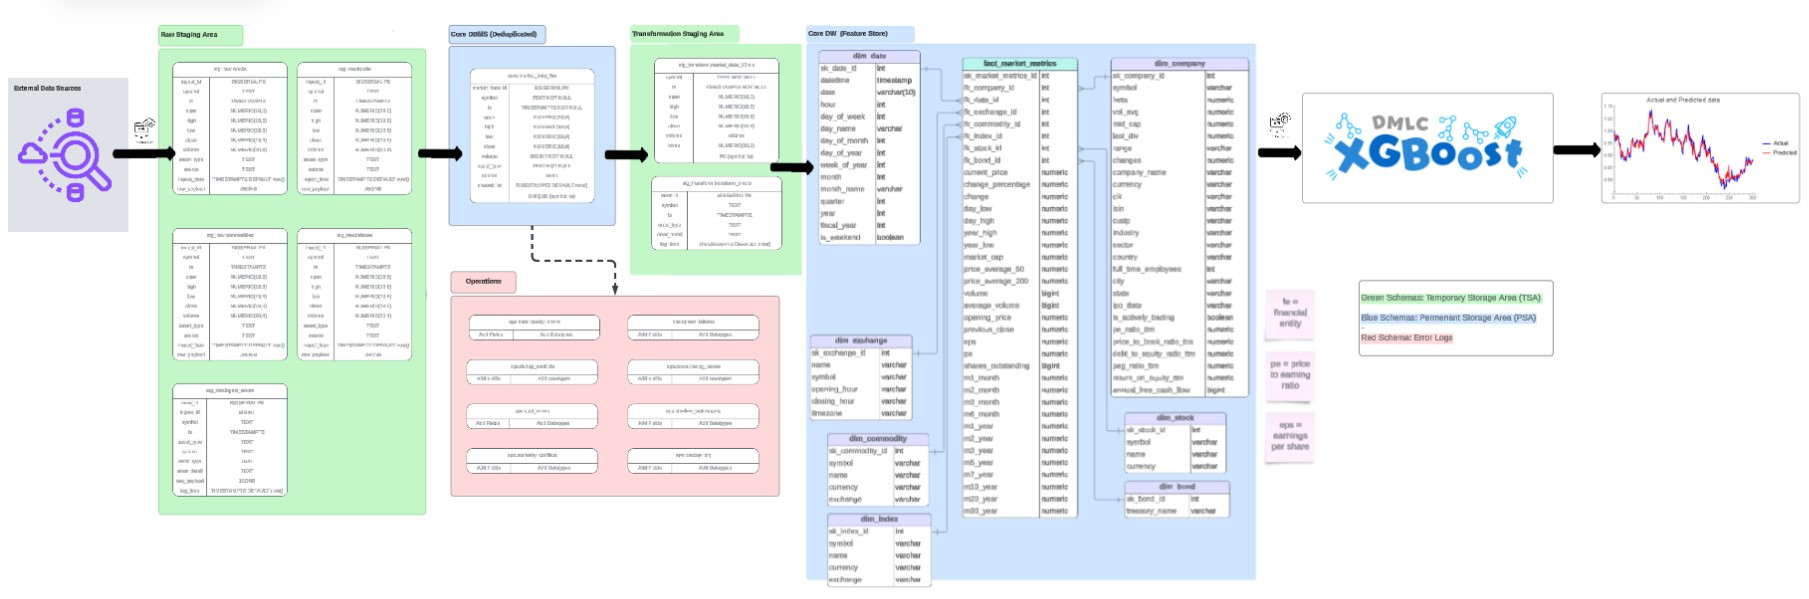
\includegraphics[width=0.95\textwidth]{images/AlgTr-ERD.jpg}
\caption{Data Flow}
\label{fig: DataFlow}
\end{figure*}

\begin{figure*}[ht]
\centering
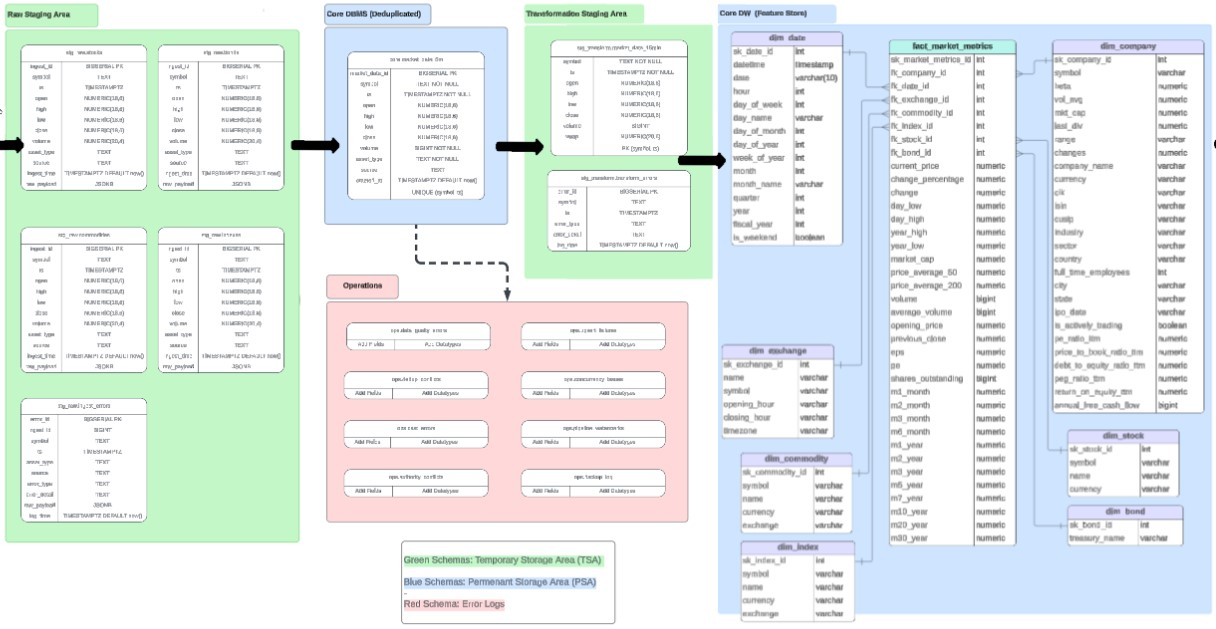
\includegraphics[width=0.95\textwidth]{images/DC_DW_ERD.jpg}
\caption{ERD for ELT}
\label{fig: ERD for ELT}
\end{figure*}

\begin{figure*}[t]
\centering
\begin{minipage}{0.44\textwidth}
    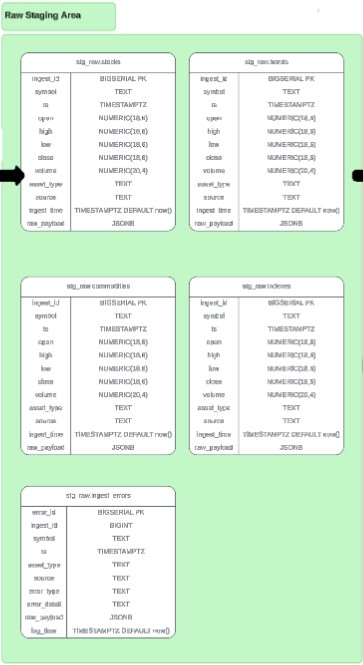
\includegraphics[width=\linewidth]{images/Raw-Staging-Area.jpg}
    \caption{Raw Staging Area}
    \label{fig:rawStaging}
\end{minipage}
\hfill
\begin{minipage}{0.52\textwidth}
    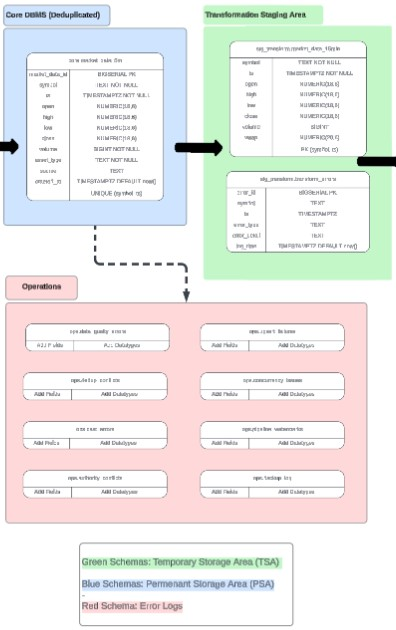
\includegraphics[width=\linewidth]{images/Core_dbms_ops_transform_staging_area.jpg}
    \caption{Core DBMS, error logs, and transformation}
    \label{fig:core_dbms}
\end{minipage}
\end{figure*}

\begin{figure*}[ht]
\centering
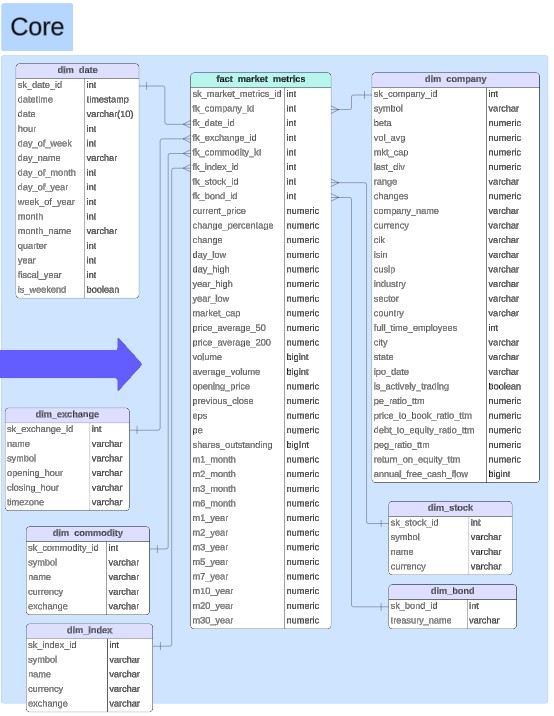
\includegraphics[width=1.0\textwidth]{images/core_dw.jpg}
\caption{Core Data Warehouse}
\label{fig: ERD for ELT}
\end{figure*}

%

% As you can see in Fig.~\ref{fig: ETL}, the data from Financial Model Prep was acquired into Staging Tables: Extract raw stock, index, bond, and commodity data from the Financial Model Prep API. Load raw data to individual staging tables—used the automatic collector described in Section~\ref{sec:DataCollection}.
            
%  From Staging Tables, data is transferred to the Model Table: Extract, transform, and merge data, then store it in the model table. Used a Jupyter Notebook.
 
%  From Model Table to Model / User Interface: Connect Model to Table; the Model will query the Table to fetch training data. The user interface will be built in the future. 
 
% From Staging Tables to Model Table in Detail: A Jupyter Notebook will extract the raw data from the staging tables, merge and transform the data and load them into a single table for model training.

% Data Cleaning: FMP's raw data contains missing entries and duplicates. The Jupyter Notebook script creates a dataframe for each dataset, removes duplicates, and uses an *** appropriate imputation method (needs further research) to fill in the missing time entries. 

% % Data Formatting: The extracted data must be formatted to align with the DW schema, including proper conversion of date formats, numerical precision, and standardization of measurement units (e.g., currency, percentages). \\ 

% Data Transformation: Only categorical values are transformed during this process. Numerical values are normalized during model training. 

% The data collection subsystem allows downloading historical data from CSV files and directly from the FMP API, and uploading them to the staging database in PostgreSQL, thereby bypassing the CSV file (Fig.~\ref{fig: ETL}).


%%%%%%%%
\section{The Automation Process Implementation for the 
         stocks-price prediction XGBoost model}
%%%%%%%%

\setlength{\fboxrule}{2pt}
    	\fcolorbox{red}{white}{
        	\parbox{0.8\linewidth}{
         -- -- This is your Subteam III Construction I and II reports. \\
        	}
        }\\

% Due to limitations of the Fir server at DRI, the virtual machine on DRI's Arbutus Cloud must execute several special scripts. Fir's \textit{crontab} tool has been disabled, and Fir has minimum requirements on job length; Arbutus Cloud provides access to scheduled tasks and has no limitations on job length. The regularity and short runtime of many scripts require large pieces of work to be done outside the Fir database, split between Arbutus Cloud and local (personal) machines. Because the databases on Fir and Arbutus Cloud are disjoint, Fir's PostgreSQL database must be initialized with historical data, then updated with current stock information from the automatic data collector running on Arbutus Cloud. 

% \subsection{Historical Stock Data Collection}
% \setlength{\fboxrule}{2pt}
%     	\fcolorbox{red}{white}{
%         	\parbox{0.8\linewidth}{
        	
%             -- James\\
%             -- Youry, please review 2025-11-27
%            }
%         }\\

% The FMP API, configured for 5-minute intraday intervals, return up to 10 days of data per stock symbol per API call. Due to the large number of API calls required, a script is needed to automate data collection across the desired date range. A Python script, running on a local machine, automates this process. The script defines a start date, an end date, and stock symbols. Then, for each stock symbol, an inner loop iterates through the target range, calling the API with distinct 5-day windows. Each time the inner loop terminates, the individual stock's results are saved locally into a CSV file named with the corresponding stock symbol. The outer loop terminates when all stock symbols have been processed. The resulting CSV files serve as input to a script that checks for missing entries. This Python date validation script loads each file based on the stock symbols defined in the data collector. Exclusion dates are inserted into a list (holidays, etc.) to avoid false alerts. The start date, end date, opening time, and closing time are also defined, matching the definitions in the historical data collection script. Expected 5-minute intervals are calculated, and then actual results are compared against the generated list. Any missing values are logged to the console for the operator to investigate. To confirm the API results were correct, missing entries are double-checked with a manual API call in a web browser. Occasionally, FMP is missing data for an interval. Still, it is critical to validate that the missing entry is a fault in FMP's data collection process and is unrelated to script execution. The raw data CSVs are ready to be patched (missing entries filled with previous entries' information, interpolated, etc.) and uploaded to the database. 

% \subsection{CSV File to Database Upload Automation}

% \setlength{\fboxrule}{2pt}
%     	\fcolorbox{red}{white}{
%         	\parbox{0.8\linewidth}{
        	
%             -- Brandon\\
%             -- Youry, please review 2025-11-25
%            }
%         }\\

% The CSV stock data is inserted into the Fir-hosted database using automated Python scripts, which are publicly available on GitHub \cite{AlgorithmicTradingPublic_2025}. An SSH Tunnel to Fir and multi-factor authentication were required to access the Fir PostgreSQL RDBMS,
% %Youry, 1Feb commented out to reduce citations
% % \cite{DRAC_SSH_MultifactorAuth}
% so the database is accessible. A stock CSV file is read into memory and is cast into the appropriate variable format for the database. Because using multiple INSERT commands can take over 10 minutes per stock due to overhead, the script uses PostgreSQL's COPY command, which performs bulk inserts and takes approximately 5 seconds per stock. The script then iterates through the remaining stock files until all data has been copied into their respective tables. 

\subsection{Current Stock Data Collection Analysis and Modelling}
% \setlength{\fboxrule}{2pt}
%     	\fcolorbox{red}{white}{
%         	\parbox{0.8\linewidth}{
        	
%             -- James\\
%             -- Youry, please review 2025-11-27
%            }
%         }\\

% To update the database with the latest stock information, the FMP API must be called repeatedly throughout the day. The virtual machine on Arbutus Cloud, running a Bash shell on AlmaLinux, provides the mechanism for automating the current data collection script. A systemd timer is configured to run every 30 minutes, covering the period from 4:00 am to 8:00 pm Eastern Standard Time, Monday through Friday. The timer's service executes a Bash script that performs the following activities in this order: activates the Python virtual environment, initializes environment variables (API key and database connection), and runs the Python data collection script described in Section III. 



% The raw data in the staging area is transformed into a single table, appropriate for the ML model. This table contains only numerical data, as ML models are highly mathematical in nature. The number of stocks in the staging area requires a repeatable transformation process.

% The raw data is queried from the database and sent to DRI's Arbutus Cloud for Processing with a Python script. Processing is performed in Python due to the extensive libraries that facilitate data transformation. These libraries include pandas, holidays, and yfinance. Sector data is queried from yfinance for each stock and stored in a table. Each stock's data is read from the table and joined with the sector data using pandas. Commodity, bond, and index data are read in and joined to each stock on the date column. The holidays library retrieves a list of holiday dates to assess how pre-holiday and post-holiday periods affect the market. The date column is split into month, week, day, hour, and minute columns. To prevent ML models from inferring a relationship between different integer values in a single column, the script uses one-hot encoding. This technique allows the script to split the original column into a set of Boolean columns for each value present in the data. 

% \begin{lstlisting}[language=Python, caption={One-hot Encoding}, label={lst:Transformation_encoding}]
% def one_hot(og_df, feature_to_encode):
%     "Function that takes a dataframe, and a feature to one-hot encode and returns the dataframe with that feature encoded"
%     dummies = pd.get_dummies(og_df[feature_to_encode], prefix = feature_to_encode, prefix_sep = "_")
%     df = pd.concat([og_df, dummies], axis=1)
%     df = df.drop([feature_to_encode], axis=1)
%     return df
% \end{lstlisting}



% AlmaLinux provides the \textit{firewalld} service to manage port access. After opening the default PostgreSQL port, a public and private SSH key pair was generated and saved locally on the Arbutus VM. The ssh-copy-id command copies the public SSH key to Fir. A secure SSH tunnel to the Fir database is opened, using a non-dedicated port on the Arbutus VM as a local port. Finally, once the port forwarding is set up, the Arbutus terminal runs psql via the now-open SSH tunnel. This completes the connection, and the VM has command-line access to the PostgreSQL database on Fir. A limiting factor of this method is the requirement for two-factor authentication for every Fir database connection. Future work for this section includes discussions with the Digital Research Alliance of Canada to resolve the two-factor authentication issue. Preferably, a connection from Arbutus to Fir will be established exclusively through internal DRAC tools or networks, rather than via SSH, which always requires Duo authentication. Another possibility is a persistent SSH tunnel, although a connection timeout that forces re-authentication is also possible. The script to automatically insert rows has not yet been completed, but database access has been established, enabling fully automated database synchronization.

% \subsection{Testing Data Analysis Using new API from DW to Jupyter Notebook}

% The Fir cluster, which offers high-performance computing using GPUs, provides access to JupyterHub and JupyterLab for short tasks such as model training and testing. To access JupyterHub through the Fir server and use its GPUs, login through this link: \href{https://jupyterhub.fir.alliancecan.ca/}{https://jupyterhub.fir.alliancecan.ca/}.

% The model Notebook is uploaded to JupyterHub through the Fir Server. The model table is located in the Fir cluster to ensure the model can easily access it. The model uses the psycopg2 and sqlalchemy packages to connect to the database and query the model table. 

% \begin{lstlisting}[language=Python, caption={Database to Notebook Connection}, label={lst:Database to Notebook Connection}]

% engine = create_engine(f'postgresql://{username}:
%     {password}@{host}:{port}/{database_name}')

% query = "SELECT * FROM market.modelfeatures WHERE symbol IN ('AAPL', 'TSLA', 'MSFT')"

% df = pd.read_sql(query, engine)

% \end{lstlisting}

The model uses the pandas library to store the query data into a dataframe and uses the dataframe to train and predict the stock prices. The prediction results are stored and displayed on graphs. 

% \section{Future Works}

\setlength{\fboxrule}{2pt}
% This ETL and Automation system prototype can be used alongside the ML algorithm as a better data pipeline for forecasting. 
% In future research, 
% we will use 30 years of financial data for the training and testing models. DRA provides production performance training and offers an array of cutting-edge tools and resources that are crucial for enhancing the scope and impact of our research. The DRAC supports researchers across various fields by providing access to high-performance computing, data storage, and specialized software platforms that facilitate large-scale data analysis, computational modelling, and collaborative research. In support of our initiative, our team has been honoured to be selected as part of the DRI Champions Program \cite{drichamp}. This includes a research grant for 2024--2025, from which a portion of the funding is specifically allocated to promoting the DRI, supporting research activities, and providing resources to facilitate this project's continued development and growth.

\section{Project Summary and Discussion}


\section{Conclusion}

% This research paper described and discussed a new approach to data collection from FMP data sources for training, testing, and stock forecasting using XGBoost (eXtreme Gradient Boosting), an open-source, high-performance machine learning library that implements optimized gradient boosted decision trees. The new and historical datasets were uploaded to a PostgreSQL general-purpose DBMS within the DRI research project. The research team designed and tested a new API that provides direct access to the DBMS from the core subsystem for machine learning (ML) training, testing, and forecasting on the vast datasets collected, transformed, and stored in the DBMS. 

\section{Future Work and Development}

\section*{Acknowledgements}
We thank Okanagan College and the Okanagan College's (OC's) Grants-in-Aid (GIA) Committee for funding and financial support of the applied student research projects. Additionally, we would like to thank the DRA of Canada for the DRI Champions Award. 

The authors used an AI-based language tool to assist with documentation organization, grammar refinement, and clarification of written content. The AI tool did not contribute to the research design, methodology, experiments, analysis, or conclusions. All intellectual contributions and technical decisions are solely those of the authors. Entity Relationship Diagrams (ERD) were created using Lucidchart.

\section*{Appendixes}
\subsection*{Appendix I}
\subsection*{Appendix II}
\subsection*{Appendix III}

\balance

\bibliographystyle{IEEEtran}

\bibliography{AlgTr,Youry,TempBib,2026-AlgTr}
% ,TempBib

\end{document}